\chapter{Evaluation of barcode detection}
\label{sec:Evaluation of barcode detection}
Here is a compilation of the evaluation that has been made for different methods for detections of barcodes. First some results from the different features are evaluated individually regarding their accuracy. Then the accuracy and the speed of the whole system is evaluated.

To get a measure of the accuracy of the system the number of true detections and the number of false detections are calculated and plotted. There are a lot of parameters and variation of the preprocessing of the tiles that will affect the result:

 \begin{itemize}
 	\item Size of the tiles
 	\item Use of overlapping tiles or not
 	\item Use of down sampling
 	\item $\varphi$ from the algorithm in figure \ref{AdaBoost}
 	\item Use of Laplace filtering 
 \end{itemize}

In the evaluation 265 images has been used containing 1D-codes and 2D-codes. Of them 100 has been used for training and 165 for testing.

\section{Calculation of ground truth}
\label{sec:Calculation of ground truth}
One of the problems that can occur with too big tiles and when if the down sampling is too high is that the ground truth is not calculated correctly. Since 70\% of the tile has to be inside the code area there is a chance some codes will be missed out entirely. This is primarily the case for the 1D-codes since some of them are very thin. There are not really any good way to evaluate this except pick out some difficult images and look at the result. If the the tile size is too big to detect some of the codes one solution is to make them overlap with each outer. 

In the table below some tile sizes have been tried out with different down sampling. The values written in the table is how much overlap of the tiles which is necessary to achieve an acceptable result. The places in the table which is empty are cases when it's not possible to get a good result.

\begin{table}[H]
\begin{center}
     \begin{tabular}{ | l | l | l | l | l | p{5cm} |}
     \hline
     tile size & no down sample & down sample 2 & down sample 3 & down sample 4 \\ \hline
   	 24x24 & 1 & 1-2 & 3 & 	\\ \hline
     32x32 & 1 & 2-3 &   & 	\\ \hline
     48x48 & 2 &     &   &  \\ \hline
     64x64 & 3 &     &   &	\\ \hline
     \end{tabular}
\end{center}
\caption{Necessary overlap of the tiles to calculate ground truth}
\end{table}

\section{Evaluation of features}
\label{sec:Evaluation of features}
Here is an evaluation of each feature that are used in the cascade. The objective is to keep as many true tiles as possible in each step of the cascade and in the same time reduce the amount of date as much as possible. In this evaluation the objective has been to preserve at least 98\% of the true tiles in each step. Here different tile sizes and different amount of down sampling have been tried and best value of $\varphi$ has been calculated to preserve 98\% of the true tiles and as few false tiles as possible. Here only cases which gave a good result in the evaluation of the ground truth above are tested. 

\subsection{Standard deviation}
When using standard deviation the images have been preprocessed with Laplace filtering and no overlapping tiles. It has been trained on both 1D- and 2D-codes. 

\begin{table}[H]
\begin{center}
     \begin{tabular}{ | l | l | l | l | l |}
     \hline
     tile size & no down sample & down sample 2 & down sample 3 \\ \hline
   	 24x24 & 4 & 4 & 4 			\\ \hline
     32x32 & 4 & 4  & 			\\ \hline
     48x48 & 3 &     &  		\\ \hline
     64x64 & 3 &     &			\\ \hline
     \end{tabular}
\end{center}
\caption{Lowest value of $\varphi$ that keeps at least 98\% of the true tiles when using standard deviation}
\end{table}

\begin{table}[H]
\begin{center}
     \begin{tabular}{ | l | l | l | l | l |}
     \hline
     tile size & no down sample & down sample 2 & down sample 3 \\ \hline
   	 24x24 & 280 & 12.23 & 33.6 	\\ \hline
     32x32 & 96.27 & 163 & 			\\ \hline
     48x48 & 77    &     &  		\\ \hline
     64x64 & 69     &     &			\\ \hline
     \end{tabular}
\end{center}
\caption{The average number of false detection per image using standard deviation}
\end{table}

\subsection{Structure tensor}
When using structure tensor the images have been preprocessed with Laplace filtering and no overlapping tiles. It has been trained only on 1D-codes. 

\begin{table}[H]
\begin{center}
     \begin{tabular}{ | l | l | l | l | l |}
     \hline
     tile size & no down sample & down sample 2 & down sample 3 \\ \hline
   	 24x24 & 1.5-2 & 2.5 & bad result 	\\ \hline
     32x32 & 1 & 2  & 					\\ \hline
     48x48 & 1.5 &     &  				\\ \hline
     64x64 & 1 &     &					\\ \hline
     \end{tabular}
\end{center}
\caption{Lowest value of $\varphi$ that keeps at least 98\% of the true tiles when using structure tensor}
\end{table}

\begin{table}[H]
\begin{center}
     \begin{tabular}{ | l | l | l | l | l |}
     \hline
     tile size & no down sample & down sample 2 & down sample 3 \\ \hline
   	 24x24 & 226 & 121 & bad result 	\\ \hline
     32x32 & 92 & 228 & 				\\ \hline
     48x48 & 23    &     &  			\\ \hline
     64x64 & 28     &     &				\\ \hline
     \end{tabular}
\end{center}
\caption{The average number of false detection per image using structure tensor}
\end{table}

\subsection{Distance map}
The distance map is trained only with 1D-codes and without Laplace filtering.

\begin{table}[H]
\begin{center}
     \begin{tabular}{ | l | l | l | l | l |}
     \hline
     tile size & no down sample & down sample 2 & down sample 3 \\ \hline
   	 24x24 & 1 & 1.5 & 2 		\\ \hline
     32x32 & 1 & 1.5  & 		\\ \hline
     48x48 & 1 &     &  		\\ \hline
     64x64 & 1.2 &     &		\\ \hline
     \end{tabular}
\end{center}
\caption{Lowest value of $\varphi$ that keeps at least 98\% of the true tiles when using distance map}
\end{table}

\begin{table}[H]
\begin{center}
     \begin{tabular}{ | l | l | l | l | l |}
     \hline
     tile size & no down sample & down sample 2 & down sample 3 \\ \hline
   	 24x24 & 90 & 15 & 71 	    \\ \hline
     32x32 & 35 & 23 & 			\\ \hline
     48x48 & 45    &     &  	\\ \hline
     64x64 & 52     &     &		\\ \hline
     \end{tabular}
\end{center}
\caption{The average number of false detection per image using distance map}
\end{table}


\subsection{FAST corner detection}
The FAST corner detection feature is trained only with 2D-codes and without Laplace filtering. When down sampling with 3 the result seems to drop significantly, then it seems like it detects a lot of corners in the 1D-code.

\begin{table}[H]
\begin{center}
     \begin{tabular}{ | l | l | l | l | l |}
     \hline
     tile size & no down sample & down sample 2 & down sample 3 \\ \hline
   	 24x24 & 1.5 & 4 & 3 		\\ \hline
     32x32 & 3 & 4 & 			\\ \hline
     48x48 & 2.2 &     &  		\\ \hline
     64x64 & 3 &     &			\\ \hline
     \end{tabular}
\end{center}
\caption{Lowest value of $\varphi$ that keeps at least 98\% of the true tiles when using FAST corner detection}
\end{table}

\begin{table}[H]
\begin{center}
     \begin{tabular}{ | l | l | l | l | l |}
     \hline
     tile size & no down sample & down sample 2 & down sample 3 \\ \hline
   	 24x24 & 75 & 17 & 138		\\ \hline
     32x32 & 59 & 21 & 			\\ \hline
     48x48 & 80    &     &  	\\ \hline
     64x64 & 44     &     &		\\ \hline
     \end{tabular}
\end{center}
\caption{The average number of false detection per image using FAST corner detection}
\end{table}

\subsection{Local binary pattern}
The LBP feature is trained only with 2D-codes and without Laplace filtering. The evaluation was in this case done together with the cascade. The reason for this is that it takes too long to test this features for all data. When using the cascade the data is reduced a lot before the step where the LBP is used. Also the training was done with 50 weak classifiers instead of 100.

\begin{table}[H]
\begin{center}
     \begin{tabular}{ | l | l | l | l | l |}
     \hline
     tile size & no down sample & down sample 2 & down sample 3 \\ \hline
   	 24x24 &  & 3 & 		\\ \hline
     32x32 &  & 2 & 			\\ \hline
     48x48 & 2 &     &  		\\ \hline
     64x64 & 2 &     &			\\ \hline
     \end{tabular}
\end{center}
\caption{Lowest value of $\varphi$ that keeps at least 98\% of the true tiles when using LBP}
\end{table}


\section{Evaluation of cascade}
\label{sec:Evalutaion of cascade}
Here are some conclusions that can be drawn from the evaluation of the features before evaluating the cascade.

\begin{itemize}
\item There is no reason to use tiles with sizes 24x24 and 32x32 without down sampling with 2, since all feature seems to work in this case.

\item To down sample with more than 2 seems to give really bad results with structure tensor.

\item The cascade will be a lot faster with down sampling with 2 and tile sizes 24x24 and 32x32. This is because the amount of false tiles when using standard deviation are very low.
\end{itemize}

From these conclusions the evaluation of the cascade will be done for four different cases regarding the tile size, the down sampling and the overlap of the tiles. Also the cascades has been evaluated for the two different variants which was described in \ref{sec:Cascade}. Here is the result from cascade 1.

\begin{table}[H]
\begin{center}
     \begin{tabular}{ | p{3cm} | l | p{3cm} | p{2cm}|}
     \hline
      	& ms/image & true detections in percent & false tiles \newline per image \\ \hline
   	 tile size 24x24 \newline down sampling 2 \newline overlap 1 
   	 & 75 & 1D: 98 \newline 2D: 95 & 1D: 0.7 \newline 2D: 0.14 				\\ \hline
     tile size 32x32 \newline down sampling 2 \newline overlap 2 
     & 190 & 1D: 98 \newline 2D: 93 & 1D: 0.26 \newline 2D: 0				\\ \hline
     tile size 48x48 \newline down sampling 1 \newline overlap 2 
     & 420    & 1D: 96 \newline 2D: 94.5 & 1D: 0.3 \newline 2D: 0.097
     \\ \hline
     tile size 64x64 \newline down sampling 1 \newline overlap 3 
     & 631 & 1D: 0.96 \newline 2D: 0.93 & 1D: 0.35 \newline 2D: 0.93		 \\ \hline
     \end{tabular}
\end{center}
\caption{Result from evaluation of cascade 1}
\end{table}

Here is the evaluation of cascade 2.
\begin{table}[H]
\begin{center}
     \begin{tabular}{ | p{3cm} | l | p{3cm} | p{2cm}|}
     \hline
      	& ms/image & true detections in percent & false tiles \newline per image \\ \hline
   	 tile size 24x24 \newline down sampling 2 \newline overlap 1 
   	 & 74 & 1D: 96 \newline 2D: 95 & 1D: 0.5 \newline 2D: 0.12 				\\ \hline
     tile size 32x32 \newline down sampling 2 \newline overlap 2 
     & 210 & 1D: 97 \newline 2D: 94 & 1D: 0.18 \newline 2D: 0				\\ \hline
     tile size 48x48 \newline down sampling 1 \newline overlap 2 
     & 390    & 1D: 96 \newline 2D: 94.5 & 1D: 0.02 \newline 2D: 0.097
     \\ \hline
     tile size 64x64 \newline down sampling 1 \newline overlap 3 
     & 630 & 1D: 0.96 \newline 2D: 0.93 & 1D: 0.18 \newline 2D: 0		 \\ \hline
     \end{tabular}
\end{center}
\caption{Result from evaluation of cascade 2}
\end{table}

Bellow is the result from the first two tests of cascade 1 (first two row in table 7.11).
\begin{figure}[H]
\centering
	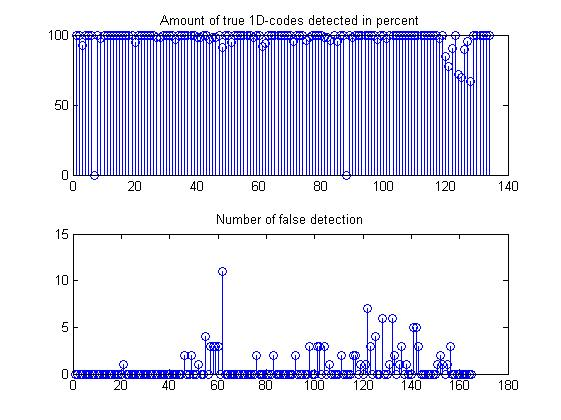
\includegraphics[scale=0.5]{Result24x24_1D}
	\caption{Result for 1D-codes from evaluation of cascade using tile size 24x24, down sampling 2, and no overlap}
	\label{Result24x24_1D}
\end{figure}

\begin{figure}[H]
\centering
	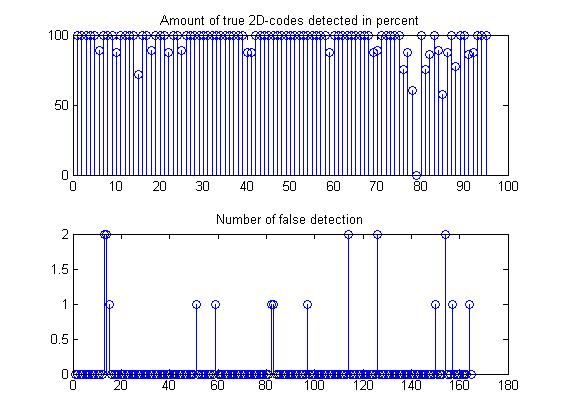
\includegraphics[scale=0.5]{Result24x24_2D}
	\caption{Result for 2D-codes from evaluation of cascade using tile size 24x24, down sampling 2, and no overlap}
	\label{Result24x24_2D}
\end{figure}

\begin{figure}[H]
\centering
	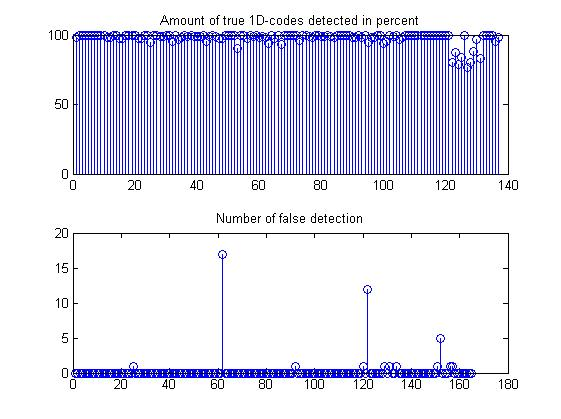
\includegraphics[scale=0.5]{Result32x32_1D}
	\caption{Result for 1D-codes from evaluation of cascade using tile size 32x32, down sampling 2, and overlap 2}
	\label{Result32x32_1D}
\end{figure}

\begin{figure}[H]
\centering
	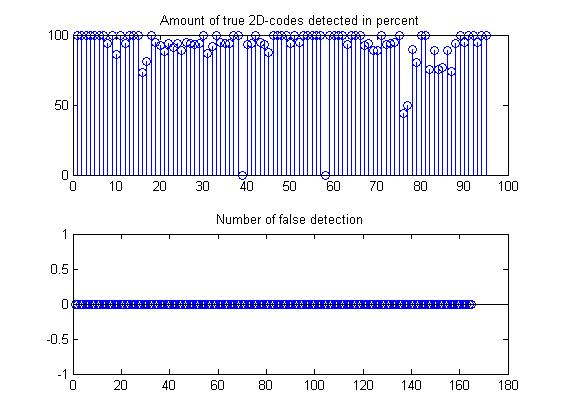
\includegraphics[scale=0.5]{Result32x32_2D}
	\caption{Result for 2D-codes from evaluation of cascade using tile size 24x24, down sampling 2, and no overlap}
	\label{Result24x24_2D}
\end{figure}

\begin{figure}[H]
\centering
	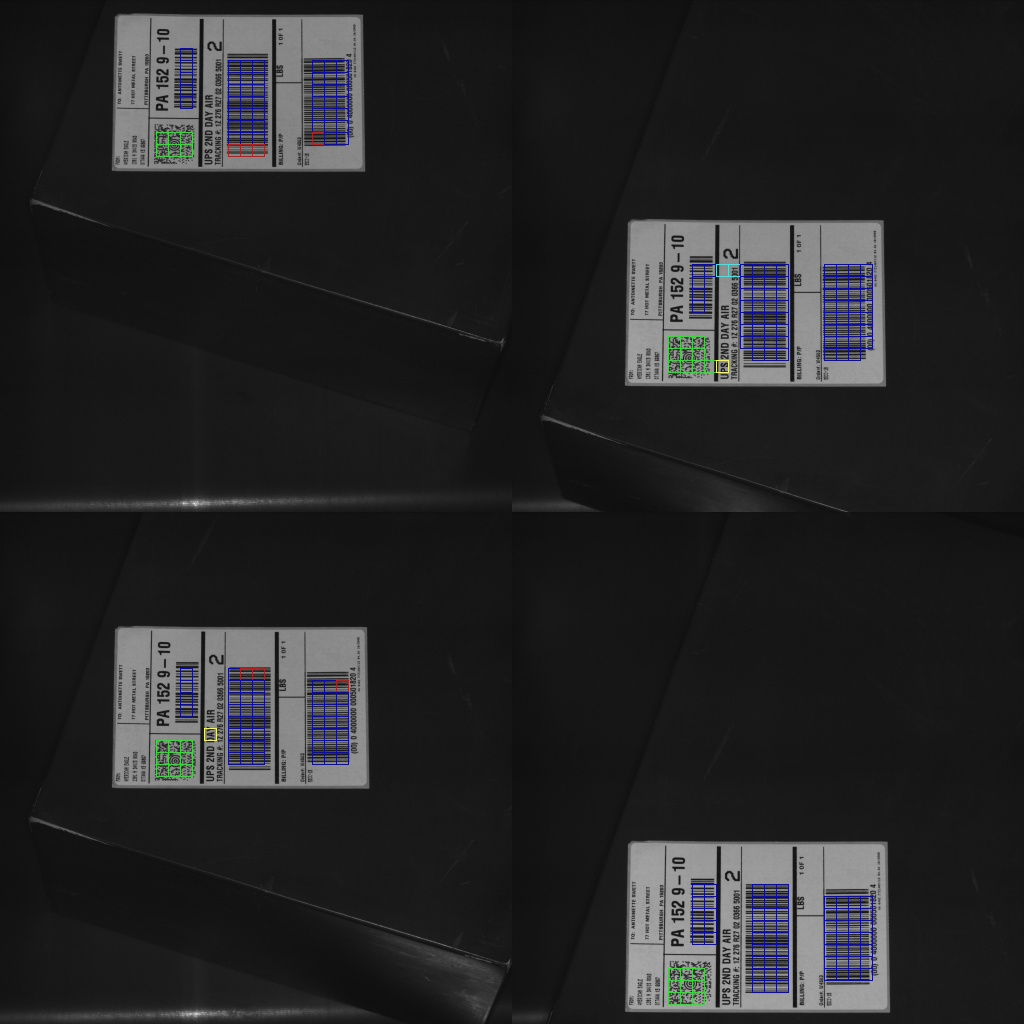
\includegraphics[scale=0.25]{Result24x24}
	\caption{Result from evaluation of cascade using tile size 32x32, down sampling 2, and overlap 2}
	\label{Result32x32}
\end{figure}

\section{Conclusions}
\label{sec:Conclusions}
The two variants of the cascade gave rather similar results. Both the structure tensor and the FAST corner detection are rather good at distinguish between 1D- and 2D-codes.

The first two cases (the two first rows in table 7.11 and table 7.12) gives overall better result, especially regarding the speed. Which one of them that is best depend depend of what is required of the system, regarding speed and accuracy.

One alternative is to omit the distance map feature in the cascade and only use standard deviation and structure tensor for detection of 1D-codes. The result is still rather good, the amount of true detections is even higher but the amount of false tiles will increase.

The amount of true tiles detected can in some cases seem a bit weak, especially for 2D-codes. In the upper graph in \ref{Result24x24_2D} one can see that in one image there are no detections at all. This is the case when the codes are at the border of the image and only a small part are inside. Since in this case only a few tiles will cover the codes there is a big chance that these will be lost in the post-processing. The alternative is to reduce the amount of post-processing but this will instead lead to more false tiles.  

% Local Variables:
% TeX-master: "main.tex"
% End:
